%Indice

%Premessa
%Cenni storici
%Descrizione Firewall Galliera
%Migrazione FW interno
%  Simulazione con lxc
%  Sistemi di automazione
%Il futuro
%  {\em iptables}
%  eBPF/XDP

\chapter{Introduzione} % Main chapter title

\label{Chapter1} % For referencing the chapter elsewhere, use \ref{Chapter1} 

%----------------------------------------------------------------------------------------

% Define some commands to keep the formatting separated from the content 
\newcommand{\keyword}[1]{\textbf{#1}}
\newcommand{\tabhead}[1]{\textbf{#1}}
\newcommand{\code}[1]{\texttt{#1}}
\newcommand{\file}[1]{\texttt{\bfseries#1}}
\newcommand{\option}[1]{\texttt{\itshape#1}}

%----------------------------------------------------------------------------------------

Il progetto che \`e stato realizzato ha avuto origine da considerazioni
relative alla necessit\`a di aggiornare il sistema di firewall a protezione
della rete interna dell'ospedale Galliera.

La LAN dell'ospedale \`e connessa ad internet dal 1996 e sin da allora il
traffico di rete da e verso l'esterno \`e stato regolato e monitorato da
router/firewall Linux da me opportunamente configurati.

Nel tempo le esigenze di connettivit\`a sono via via aumentate ed i nostri
sistemi si sono dimostrati adeguati sia per quanto riguarda le funzionalit\`a
che per prestazioni.

Tuttavia nell'arco del 2017 si sono presentate alcune situazioni di
criticit\`a, dovute sostanzialmente al grande numero di regole sui firewall.

Pur essendo riuscito a risolvere i problemi ho ritenuto di dover considerare
questi segnali di possibile obsolescenza del sistema, studiando le attuali
alternative agli strumenti scelti oramai circa 17 anni fa: cio\`e in pratica
le alternative ad {\em iptables}.  In effetti l'alternativa c'\`e: si chiama
nftables ed il suo scopo è proprio quello di soppiantare {\em iptables}
superandone tutte le limitazioni.

Il progetto di migrazione da {\em iptables} a nftables \`e consistito prima di
tutto nello studio del nuovo sistema, nella riorganizzazione delle regole dei
due firewall (operazione ancora in corso), e nella preparazione di scenari di
test usando macchine virtuali.

\chapter{}
Nel frattempo l'analisi dello stato delle cose del kernel Linux ha evidenziato
una recente presa di posizione di molti, tra cui importanti sviluppatori e
aziende, che sostiene l'impossibilit\`a di elim

Netfilter è un framework implementato da Linux che permette di
compiere diverse operazioni relative al traffico di rete: packet-filtering,
nat, mangling, etc.

I predecessori di iftables sono stati {\em ipfwadm} per i kernel dall'1.2.x (con x>0)
al 2.0.x (1995-1999), {\em ipchains} per i kernel 2.2.x (1999-2001).  {\em iptables} è
presente dal kernel 2.4.x in poi (2001).

L'attuale (2018) kernel è il 4.15.9 e tuttora, su Linux, {\em iptables} è lo
strumento di packet-filtering più utilizzato sia come firewall limitato al
singolo host, sia per la protezione di sotto-reti e per la realizzazione di
diverse soluzioni che richiedano analisi, classificazione, elaborazione e
modifica di pacchetti di rete in transito.

{\em iptables} è quindi in produzione da cira 17 anni anche se, a partire dalla
versione di kernel 3.13 (gennaio 2014
https://kernelnewbies.org/Linux\_3.13\#nftables.2C\_the\_successor\_of\_{\em iptables}),
Linux offre uno nuovo strumento alternativo ad {\em iptables}: nftables. Nftables
appare per la prima volta nel 2009 (https://lwn.net/Articles/564095/) ma il
progetto langue fino al 2014 quando torna ad attirare l'attenzione degli
sviluppatori interessati a sopperire ai difetti di progettazione e alle carenze
di {\em iptables}.

{\em iptables} è composto in realtà da un insieme di componenti separate e ognuna di
esse ha consapevolezza del singolo protocollo che gestisce ― ipv4, ipv6,
Ethernet bridging, ARP - il codice è quindi replicato quattro volte.

Questa situazione è frustrante per gli sviluppatori e l'idea di un nuovo
sistema di packet filtering unico e /general purpose/ rende accettabile lo
sforzo necessario all'introduzione di un'ulteriore macchina virtuale (VM) nel
kernel.

L'idea di una VM che esegua bytecode nel kernel potrebbe sembrare, dal punto di
vista delle prestazioni, un errore; tuttavia ci si rende invece conto che il
bytecode può offrire prestazioni migliori del codice che sostituisce.  Inoltre
nftables introduce sostanziali miglioramenti rispetto al predecessore.

Quel che succede però è che nftables non rimpiazza {\em iptables}: lo affianca.  A
differenza dei suoi predecessori non esiste quindi una versione di kernel a
partire dalla quale il vecchio sistema non è più supportato.

Uno dei motivi, a mio parere uno dei principali, per cui nftables non ha
soppiantato da un giorno all'altro {\em iptables} consiste nella vasta adozione di
{\em iptables} a tutti i livelli, dai singoli host, ai dispositivi (cosiddetti IoT) e
soprattutto nei grandi datacenter (cloud).

\chapter{Cenni storici}

\label{Cenni storici} % For referencing the chapter elsewhere, use \ref{Chapter1} 

Per inquadrare l'argomento Linux firewall ritengo possa essere interessante
fornire un breve riassunto dell'evoluzione degli strumenti per la
classificazione ed il filtraggio dei pacchetti nel kernel Linux. Nella tabella \ref{tab:history}
vengono considerate solo i rilasci nei kernel stabili. Fino alla serie 2.6.x le
nuove fetures venivano introdotte sperimentalmente nelle versioni con major
revision number dispari, ad esempio 2.3.4; dalla versione 3 questo cambia e non
esiste più la differenza tra kernel sperimentale e di produzione.

\begin{center}
  \label{tab:history}
  \begin{table}[ht]
    \centering % used for centering table
      \begin{tabular}{@{}llcc@{}}
     \toprule
     {\bf Framework/tool} &         {\bf Anno}      &  {\bf Kernel} & {\bf Coder}\\ \midrule
         ipfw     & 1994      & 1.0  & Alan Cox \\
         ipfwadm  & 1995-1999 & 1.2.$x$\marginnote{con $x>0$} - 2.0 & A.  Cox e Jon Vos\\ [0.5ex]
         ipchains & 1999-2001 & 2.2  & Rusty Russell \\ [0.5ex]
         iptables & 2001-     & 2.4  & Rusty Russell \\ [0.5ex]
         nftables & 2014-     & 3.13 & gli stessi di iptables \\ [0.5ex]
         eBPF/XDP &           &      & \\ \bottomrule
      \end{tabular}  
    \caption{Evoluzione dei tool (kernel stable)} % title of Table
  \end{table}
\end{center}
Le prime funzionalità di firewall sono state introdotte nel nel 1994 grazie al
lavoro di Alan Cox che ne ha fatto il porting da BSD.

Questo codice costituisce la prima versione delle funzionalità di firewall
all'interno del kernel Linux. Il successivo passo evolutivo, dopo ipfw, è
stato {\em ipfwadm}, in realtà una riscrittura del corrispondente {\em ipfw}
di BSD da parte di Alan Cox e Jos Vos.

Ipfw e ipfwadm consentivano di realizzare funzioni di base di un firewall:

\begin{itemize}
    \item accounting di pacchetti IP,
    \item firewall di ingresso,
    \item firewall di uscita,
    \item firewall di inoltro,
    \item redirezione (permette proxy trasparente)
    \item masquerading
\end{itemize}

A partire dal kernel Linux 2.2 (1999) viene rilasciato un nuovo sistema di packet
filtering: {\em ipchains}. Ipchains \`e sostanzialmente una completa
riscrittura del codice di ipfw di cui espande le funzionalità.  In particolare
ipchains gestisce ulteriori protocolli oltre a TCP, UDP e ICMP, ed inoltre è
in grado di gestire la frammentazione dei pacchetti.

Anche ipchains come ipfwadm realizza però un firewall non stateful; l'unica
opzione che ha per decidere se accettare un pacchetto entrante consiste nel
verificare se il bit ACK \`e settato (significa che è una risposta relativa ad
una connessione già stabilita), ma questo significa fidarsi del pacchetto di
cui si deve stabilire il verdetto.  Ovviamente questa politica è inerentemente
oco sicura in quanto è facile inviare pacchetti costruiti ad arte per
superare i filtri del firewall.

Nel kernel 2.4 assistiamo nuovamente ad una completa riscrittura delle
funzionalità di filtro e firewall di Linux, viene introdotto il framework {\em
Netfilter} (comunemente noto come iptables).

Netfilter è molto più maturo rispetto ai suoi predecessori, permette di
realizzare firewall stateful con maggiori capacità di ispezione dei pacchetti
e capacità di {\em log}.

Alcune delle caratteristiche di NetFilter sono:

\begin{itemize}
    \item Statless packet filtering per IPv4 e IPV6
    \item Stateful packet filtering per IPv4 (inizialmente, in seguito
        aggiunto il supporto per IPv6 (2.6.15)
    \item Network e Port address translation (NAT e NAPT)
    \item Infrastruttura flessibile ed estendibile
    \item API per estensioni di terze parti
    \item Un gran numero di plugin/moduli
\end{itemize}

Per queste caratteristiche e per il fatto di essere software libero che riceve
grande supporto della comunità open source, i firewall basati su Linux
iniziano ad essere sviluppati anche in forma di prodotti commerciali offerti
da diverse aziende che ne forniscono supporto tecnico.

Il tool di configurazione di NetFilter, che è poi il nome col quale è noto il
framework stesso, è {\em iptables}.
In realtà gli strumenti di configurazione del framework NetFilter formano una
famiglia: oltre a iptables, che gestisce regole IPv4, esistono ip6tables per
regole IPV6, ebtables per realizzare firewall layer 2 (Linux bridge)
e arptables che lavora nello specifico su messaggi ARP.

Ai diversi tool corrispondono, nel kernel, parti di codice ad-hoc per il
specifico protocollo: IPv4, IPv6, EB, ARP.  A volte si usa anche il termine
{\em Xtables} per definire l'intero firewall.

La possibilità di aggiungere plugin ha fatto s\'i che nel tempo Xtables si
sia arricchito di molti moduli aggiuntivi.

A partire dal kernel 3.13 (2014) viene introdotto {\em nftables} con l'intento
di soppiantare iptables.  Il nuovo framework di classificazione di pacchetti
nasce con lo scopo di superare quelli che vengono considerati difetti o
carenze di iptables.

\begin{figure}[H]
\begin{center}
      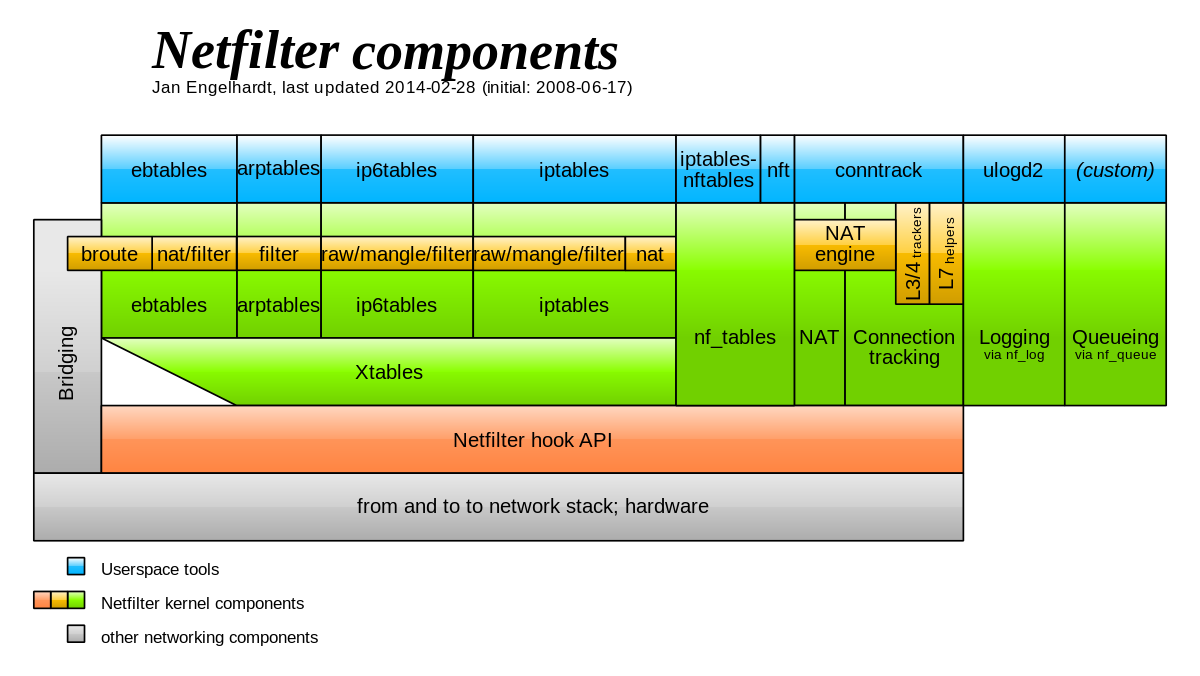
\includegraphics[width=\linewidth]{Netfilter-components.svg.png}
      \caption{Componenti di Netfilter}
      \label{fig:netfilter}
\end{center}
\end{figure}

Dalla figura \ref{fig:netfilter} risulta evidente la maggiore complessità e
ridondanza di Xtables rispetto a nftables.  Nftables riduce il numero di linee
di codice nel kernel riorganizzando e unificando quello che in iptables è
replicato per i diversi protocolli.  Inoltre nftables introduce strutture
dati, insiemi\footnote{iptables non gestisce nativamente gli insiemi ma esiste
il tool ipset che fornisce a iptables questa funzionalità}, dizionari e mappe,
che permettono di semplificare e ottimizzano le regole del firewall.
Migliorano anche la leggibilità delle regole e le prestazioni.

Un'altra caratteristica molto importante consiste nel fatto che con iptables
ogni regola viene introdotta dal comando {\em iptables} con relativi
argomenti; nftables invece consiste di un vero e proprio linguaggio nel quale
viene descritto e configurato l'intero firewall; inoltre le regole vengono
attivate atomicamente.

\chapter{Linux firewall nella rete Galliera}
\section{Cenni storici}

La LAN dell'ospedale Galliera è collegata ad internet dal 1996 e sin
dall'inizio ho utilizzato macchine Linux per i servizi di rete e per
realizzare firewall.  La prima versione, del 1996, di router/firewall l'ho
realizzata con ipfwadm.

Ad ogni evoluzione dei sistemi di firewall di Linux ho provveduto ad
aggiornare i sistemi convertendo di volta in volta le regole e approffittando
delle nuove funzionalità introdotte.  Nei casi precedenti ad nftables, la
migrazione si rendeva necessaria anche perché il vecchio framework veniva
dichiarato obsoleto e non più supportato.  Questo non è ancora accaduto per
iptables e tutto fa pensare che in questo caso il percorso sarà diverso;
vedremo in seguito i dettagli di come si possa prospettare la transizione da
iptables al suo successore (spoiler: potrebbe non essere nftables).

L'uso del firewall nei primi anni era limitato all'implementazione di filtri
per il traffico in ingresso verso i servizi esposti a internet e al {\em
masquerading} o SNAT (Source Network Address Translation) degli indirizzi IPv4
interni (di classe riservata) per l'inoltro del traffico verso internet.

\section{Architettura attuale}

Nel tempo è cresciuto il numero di sottoreti collegate, di servizi esposti e
di conseguenza la complessità delle regole configurate.

La situazione attuale consiste di due firewall Linux, uno {\em esterno} ed uno
{\em interno}.  Il firewall esterno regola il traffico tra internet, DMZ e
reti locali; quello interno regole il traffico tra le reti locali e l'esterno.

\begin{figure}
\begin{center}
      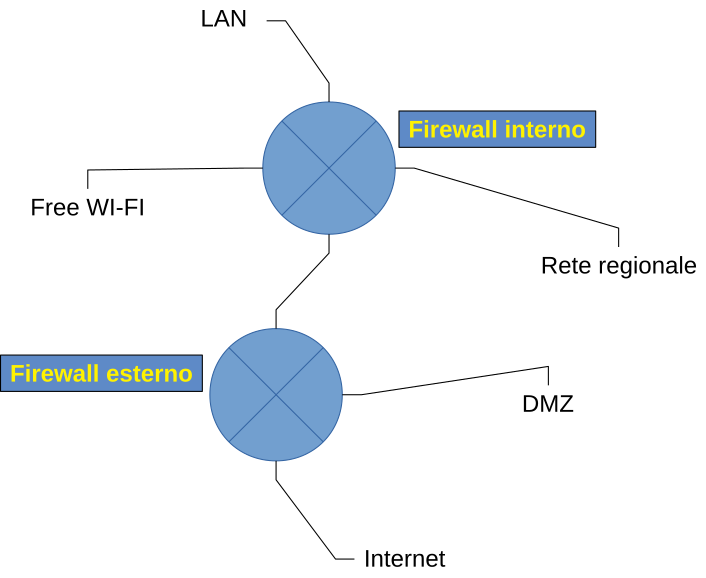
\includegraphics[width=\linewidth]{rete.png}
      \caption{Schema delle reti e dei due firewall}
      \label{fig:rete}
\end{center}
\end{figure}

In particolare sul firewall esterno sono presenti regole di tipo blacklist per
un diversi insiemi di indirizzi, che viene aggiornato
periodicamente (ogni 5 minuti).  Le liste di indirizzi provengono da:

\begin{itemize}
    \item \href{https://iplists.firehol.org/?ipset=firehol\_level1}{''FireHol
    Level1''}\footnote{https://iplists.firehol.org/?ipset=firehol\_level1} (oltre
    7000 sottoreti),
    \item \href{https://ransomwaretracker.abuse.ch/downloads/RW\_IPBL.txt}{''Ransomware
    Tracker}\footnote{https://ransomwaretracker.abuse.ch/downloads/RW\_IPBL.txt}
    (circa 400 indirizzi)
    \item {\em fail2ban} su ssh: blacklist auto-generata in base ai tentativi
    falliti di connessione via ssh (circa 9000 indirizzi al momemnto)
    \item lista di indirizzi di botnet autoprodotta da script che analizzano
    tentativi di bruteforce tipicamente su servizi di posta (oltre 12.000
    indirizzi)
\end{itemize}
 
\noindent Il totale delle regole supera le 20 mila.

Il firewall interno ha la particolarità di dover gestire le regole del {\em
captive portal}: si tratta di abilitare il traffico verso internet dei
dispositivi wireless di coloro che si sono autenticati fornando il numero di
telefono e ricevendo un codice di accesso via SMS.  Il sistema di
abilitazione, da me realizzato con la collaborazione di un collega, agisce
classificando i pacchetti in base al mac address: i pacchetti con mac adddress
abilitato vengono inoltrati regolarmente, i rimanenti vengono marcati
(l'associazione del valore al pacchetto è realizzata all'interno del kernel,
il pacchetto resta inalterato) e successivamente una regola nella catena di
inoltro devia il pacchetto verso il sito del captive portal che propone la
registrazione.

Non avendo specificato termini di scadenza la lista di mac address non
decresce mai, ad esempio al momento sono presenti oltre 23 mila indirizzi mac.

\section{Problemi dell'infrastruttura}

Nella sezione precedente ho messo in evidenza le dimensioni degli insiemi di
indirizzi e le perché proprio la gestione di così tante regole ha, durante il
2017, portato alla luce alcune carenze della soluzione implementata.

Inizialmente, infatti, per ogni indirizzo era prevista una regola
\footnote{di tipo {\em REJECT} per le blacklist e di tipo {\em RETURN} per la
gestione del wifi free},
ciò significa che prima di poter classificare ogni singolo pacchetto,
a parte ovviamente quelli subito accettati in virtù di regole relative a
traffico {\em REALTED/ESTABLISHED}.  Questo approccio basato su una regola
per ogni indirizzo risulta essere non efficace, superata una certa
soglia\footnote{nella configurazione hardware da me utilizzata questo limite
risultava essere intorno a cira 15 mila regole} risultava evidente il carico
del server Linux tanto che risultavano anche rallentati l'accesso via ssh e
l'esecuzione di comandi.

Come accennato in precedenza iptables non prevede strutture dati quali i {\em
set}, ma un framework esterno, {\em ipset}, fornisce questa funzionalità
permettendo di ridurre decine di migliaia di regole ad un unica regola (nello
specifico una regola per ogni insieme).

I problemi dovuti all'eccessivo numero di regole li ho quindi risolti usando
ipset su entrambe i firewall.  Nel caso del firewall interno è stato anche
necessario aggiornare il kernel per poter generare set contenenti mac address
in quanto questa funzionalità non è stata sempre presente.

L'introduzione di ipset ha richiesto, oltre alla modifica della configurazione
dei due firewall, anche le revisione del codice del captive portal e dei
programmi di generazione di black list.

\section{Opportunità di migrazione a nftables}

L'uso di ipset ha risolto i problemi, tuttavia ho voluto verificare cosa
comporti la migrazione da iptable a nftables, in termini di impegno necessario
rispetto ai vantaggi offerti.

Come accennato in precedenza, nftables si propone come framework completamente
nuovo, più che come evoluzione di iptables  e l'interfaccia di configurazione
è diventata un vero e proprio linguaggio di programmazione, a differenza di
iptables dove ogni regola viene inserita da un commando con relativi
argomenti.  Ci\`o significa dover riprogrammare tutte le logiche all'interno
del nuovo framwork.

\section{Confronto tra iptables e nftables}

Vediamo quali sono le principali novit\`a introdotte da nftables.
\begin{itemize}
    \item supporto nativo per dual stack IPv4 e IPv6
    \item supporto nativo per strutture dati (importanti per le prestazioni):
    set, mappe, dizionari e concatenazioni
    \item strumenti di debug e report decisamente migliori
    \item aggiunta dell'hook ingress per migliorare le prestazioni
    \item layout di regole flessibile, partendo da un insieme vuoto, rispetto
    al classico layout statico di iptables (filter/INPUT, nat/PREROUTING,
    \ldots)
    \item contatori opzionali e azioni multiple in una singola regola (ad
    esempio si pu\`o incrementare un contatore, loggare e eseguire NAT nella
    stessa regola)
    \item migliori opzioni di gestione dell'insieme di regole, aggiornamenti
    delle regole completamente atomici e incrementali
\end{itemize}

Si possono quindi inserire regole che valgono contestualemnte per IPv4 e IPv6,
mentre le strutture dati consentono di migliorare le prestazioni e la
leggibilit\`a delle regole, oltre a non richiedere il supporto di tool
esterni.

Gli strumenti di debug e log sono molto potenti, e quindi utili: \`e ad
esempio possibile tracciare l'intero percorso di un singolo pacchetto
attraverso le regole.  Esiste anche la funzione di monitor che permette di
osservare in tempo reale le modifiche alle regole di firewall.
Molto utile per la gestione è inoltre la possibilità di inserire commenti
all'interno delle regole, commenti quindi visibili interrogando il kernel e non
solo osservando il codice originale (che potrebbe nel frattempo essere stato 
modificato o andato perso).

Ad esempio, cerchiamo tra le regole attualmente in uso quelle che non
dovrebbero essere usate in produzione:
\begin{lstlisting}
# nft list ruleset | grep -w comment.\*DEBUG
ip saddr @testsources nftrace set 1 comment "DEBUG: XXX remove in production"
\end{lstlisting}

\section{Packet flow in nftables}

\begin{figure}[H]
    \centering
    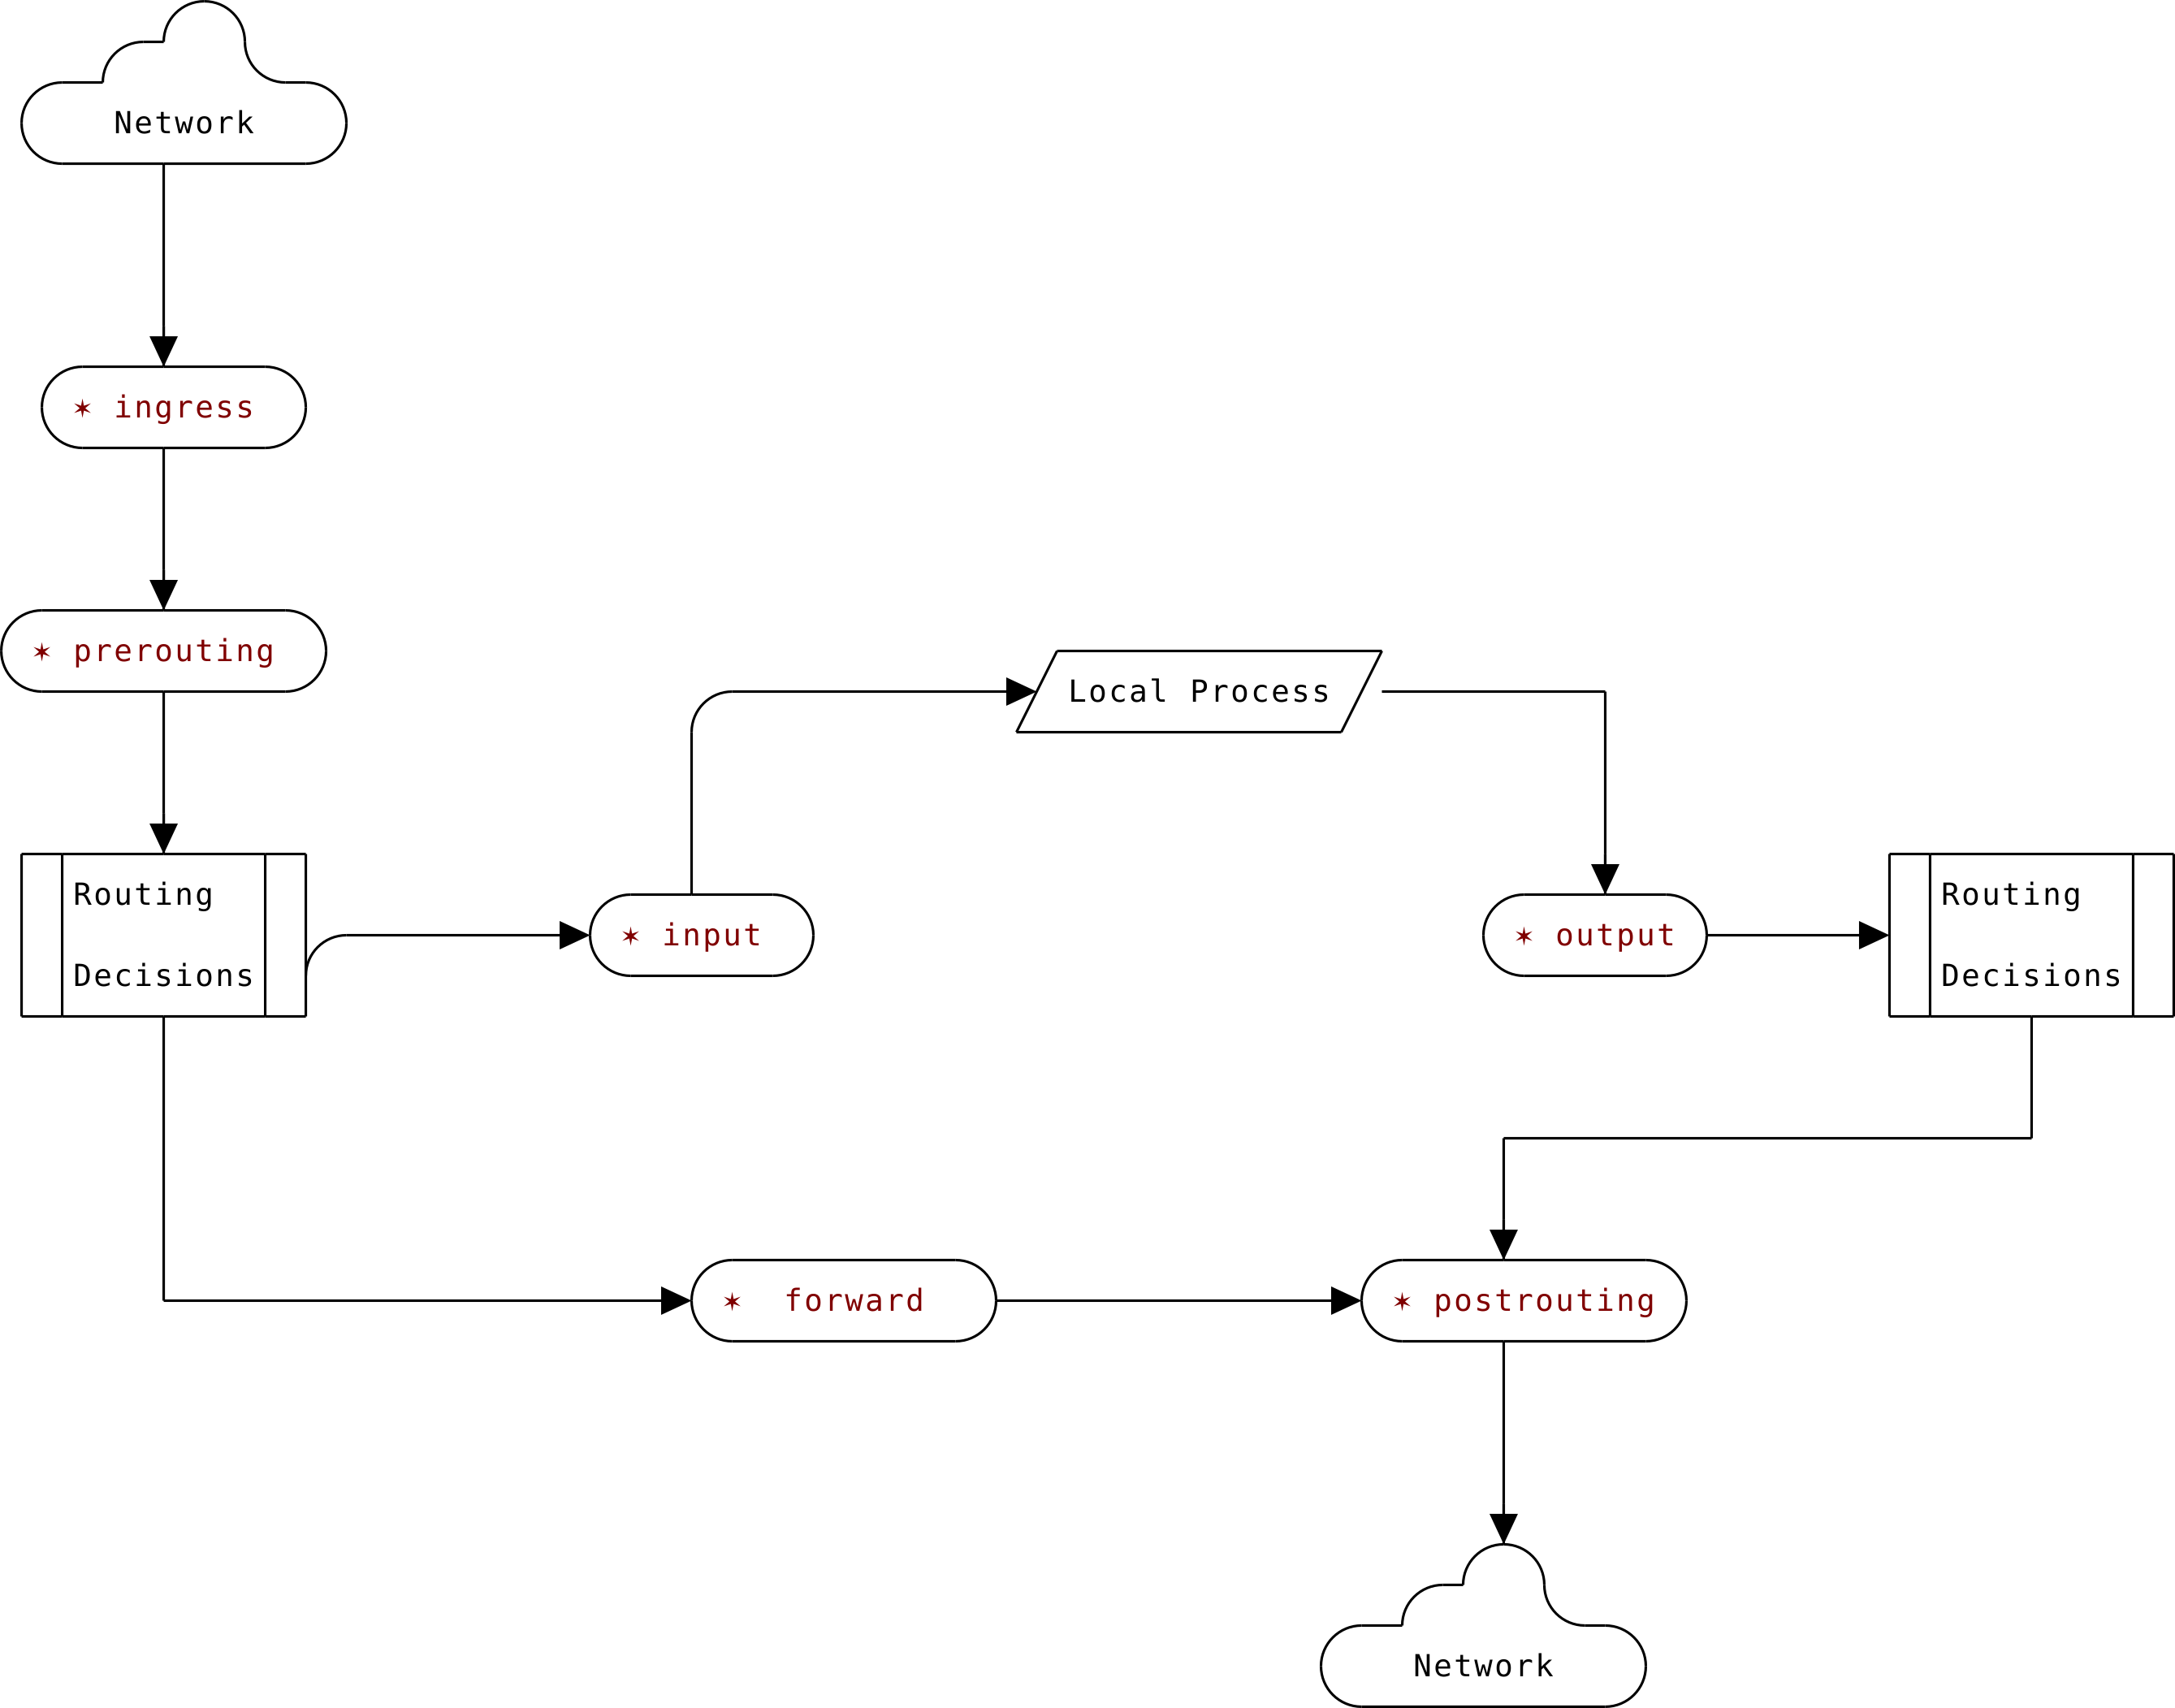
\includegraphics[width=\linewidth]{flow.svg.png}
    \caption{Schema del flusso di pacchetti in ftables}
    \label{fig:flow}
\end{figure}

%\begin{Verbatim}[fontsize=\scriptsize, fontseries=b, fontfamily=courier, samepage=false]
%    {NETWORK}
%        |
%        |
%        v                   
%    (ingress)               .----> <Local Process> ----.
%        |                   |                          |
%        |                   |                          |
%        |                   |                          |
%   (prerouting)             |                          |
%        |                   |                          |
%        |                   |                          |
%        v                   |                          v
%[Routing Decision] ----> (input)                   (output) ----> [Routing Decision]
%        |                                                                 |
%        |                                                                 |
%        |                                               .-----------------'
%        |                                               |
%        |                                               v
%        '------------------------> (forward) ----> (postrouting)
%                                                        |
%                                                        |
%                                                        |
%                                                        v
%                                                    {NETWORK}
%\end{Verbatim}

Lo schema rappresenta i possibili percorsi di un pacchetto: l'asterisco
evidenzia gli hook ai quali si possono associare le catene contenenti le
regole:
\begin{itemize}
  \item ingress
  \item prerouting
  \item input
  \item output
  \item forwarding
  \item output
  \item postrouting
\end{itemize}
\noindent La possibilit\`a di intervenire precocemente sul pacchetto, appena
passato al livello superiore dal driver della scheda di rete, \`e fondamentale
per gestire attacchi tipo DDoS: questo \`e reso possibile dall'hook ingress
che interviene prima del prerouting.

I pacchetti che destinati a qualche processo locale (cioè sono indirizzati
all'host stesso) sono gestiti tramite l'hook input ed analogamente quelli
generati da processi locali tramite l'hook output.

Il traffico che deve essere inoltrato fra le due reti viene gestito tramite
l'hook forward. Il NAT interviene in prerouting (DNAT) e postrouting (SNAT).

Il layout iniziale di nftables \`e semplicemente l'insieme vuoto,
l'amministratore \`e libero di configurare tavole (table) e catene
(chain)\footnote{Le tavole sono contenitori di catene che a loro volta
contengono regole} nel modo ritenuto pi\`u adatto al problema da risolvere.

Nemmeno i contatori sono attivi per default, a differenza di iptables, ma
devono essere esplicitamente attivati quando necessario, migliorando
cos\`i le prestazioni. Il fatto di poter indicare pi\`u azioni per una regola
rende pi\`u consistente e leggibile il codice, con
iptables spesso è necessario saltare ad un'altra catena contenente le diverse
azioni. Ad esempio, log e drop con iptables:

\begin{lstlisting}
# iptables -t filter -A OUTPUT -d 10.0.0.1 -j LOG # Log, continue to next rule
# iptables -t filter -A OUTPUT -d 10.0.0.1 -j DROP # Drops the same packet
\end{lstlisting}
oppure 
\begin{lstlisting}
# iptables -t filter -N LOGGING # Create non-base chain for logging
# iptables -t filter -A LOGGING -j LOG # Add rule to logging chain to LOG
# iptables -t filter -A LOGGING -j DROP # Add rule to logging chain to DROP
# iptables -t filter -A OUTPUT -d 10.0.0.1 -j LOGGING # Jump LOGGING if match
\end{lstlisting}
\noindent con nftables un unica regola:
\begin{lstlisting}
# nft add rule ip FILTER OUTPUT ip daddr 10.0.0.1 log drop
\end{lstlisting}

\noindent Un semplice esempio di configurazione per un server web potrebbe essere
questo:

\lstinputlisting[caption=Semplice esempio per server web, style=customc]{nftables-web.conf}

\noindent Notare, riga 9, che le connessioni già stabilite o relative a
connessioni già stabilite, informazione ricavata dalla conntrack table,
sono accettate.
I servizi raggiungibili dall'esterno sono ssh, http e https, tutto il resto
viene ignorato (drop) senza inviare "ICMP host unreachable". Inoltre i
pacchetti rifiutati vengono contati (counter).

\begin{minipage}{\linewidth}
\lstinputlisting[caption=Semplice esempio di router/firewall, style=customc]{nft-simple-forward.nft}
\end{minipage}

\noindent Questo esempio descrive il comportamento di un semplice
router/firewall. La tavola è associata ai protocolli IPv4 e IPv6 (inet) e
definisce due insiemi contenenti indirizzi dei due tipi (righe 2 e 7).
Al solito viene accettato traffico relativo a connessioni attive (riga 13)
mentre viene ignorato traffico non valido (causato da stealth port scan o da
problemi nella conntrack table o da cause benigne).
Oltre ad accettare connessioni verso qualsiasi server ssh e http(s), un
verdetto positivo è previsto anche per qualsiasi connessione verso i server
elencati ei due set.
Per ognuna delle categorie sopra elencate viene attivato il contatore.

%\begin{lstlisting}
%$ sudo iptables -A INPUT -m conntrack --ctstate ESTABLISHED,RELATED -j ACCEPT
%\end{lstlisting}

\chapter{Migrazione Captive Portal}

Lo schema di identificazione ed autorizzazione è il seguente:
\begin{enumerate}
    \item il pacchetto viene analizzato per verificare se il mac
    address è stato autorizzato
    \begin{itemize}
        \item sì: allora finisce l'analisi e il pacchetto viene inoltrato
        \item no: il pacchetto viene marcato (0x63)
    \end{itemize}
    \item in fase di prerouting, se il pacchetto è marcato ed la porta di
    destinazione è http allora viene reindirzzato (DNAT) alla pagina del
    captive portal
    \item negli altri casi (pacchetto marcato e traffico non http) allora il
    pacchetto viene scartato in fase di forwarding
\end{enumerate}

La pagina web del captive porta chiede all'utente di inserire un numero di
cellulare in suo possesso al quale invia un codice OTP via SMS. Quando
l'utente dimostra, inviandolo (POST), di essere a conoscenza del codice, il
sistema registra il suo mac address fra quelli autorizzati e salva in un
database sqlite l'associazione (mac address, numero di telefono).

La configurazione di iptables che realizza quanto descritto sopra è la
seguente:

\begin{minipage}{\linewidth}
\lstinputlisting[caption=Mangle per wifi free, style=customc,
label={lst:iptables-wifi}]{captive-iptables.conf}
\end{minipage}

\noindent Il listato \ref{lst:iptables-wifi} rappresenta la configurazione del
firewall limitatamente alle regole strettamente necessarie a realizzare la
funzionalità di captive portal. Il fatto di aver eliminato le regole non
pertinenti il caso in esame può far sembrare inutili o ridondanti alcune di
quelle elencate.

Le prime nove righe sono relative alla marcatura in fase di prerouting:
\begin{itemize}[itemindent=2em]
    \item[(riga 4)] il traffico proveniente dalla rete wifi (192.168.16.0/20)
    verrà analizzato dalla catena internet (salta alla riga 8)
    \item[(riga 8)] se il mac address sorgente è contenuto nel set captive\_ok
    ritorna
      \item[(riga 9)] marca il pacchetto con il valore 0x63 (99 decimale)
  \end{itemize}
  La tavola filter, riga 11:
  \begin{itemize}[itemindent=2em]
      \item[(riga 12)] di default scarta i pacchetti che non soddisfano una delle regole
      \item[(riga 13)] accetta il traffico relativo a connessioni già attiv
      \item[(riga 14)] scarta i pacchetti marcati con il valore 0x63
\end{itemize}
La tavola di NAT ha il compito di indirizzare il traffico http verso il sito
del captive portal.

Le righe dalla $20$ in poi sono relative all'insieme che contiene i mac
address autorizzati\footnote{gli indirizzi non sono quelli reali perché anche
il mac address è un dato personale e agli utenti non è stato notificato un uso
di questo tipo dei loro dati}: captive\_ok.
L'intestazione descrive la struttura dati di tipo hash di mac address, a
seguire tutti gli elementi dell'insieme.

Il porting di questa logica a nftables è la seguente:
\lstinputlisting[caption=Captive portal con nftables, style=customc,
label={lst:nftables-wifi}]{captive-nftables.conf}



